\documentclass[lecture,12pt,]{pcms-l}
\input preamble.tex

% For faster processing, load Matlab syntax for listings
\definecolor{MyDarkGreen}{rgb}{0.0,0.4,0.0}
\lstloadlanguages{Matlab}%
\lstset{language=Matlab,
        frame=single,
        basicstyle=\small\ttfamily,
        keywordstyle=[1]\color{Blue}\bf,
        keywordstyle=[2]\color{Purple},
        keywordstyle=[3]\color{Blue}\underbar,
        identifierstyle=,
        commentstyle=\usefont{T1}{pcr}{m}{sl}\color{MyDarkGreen}\small,
        stringstyle=\color{Purple},
        showstringspaces=false,
        tabsize=5,
        % Put standard MATLAB functions not included in the default
        % language here
        morekeywords={xlim,ylim,var,alpha,factorial,poissrnd,normpdf,normcdf},
        % Put MATLAB function parameters here
        morekeywords=[2]{on, off, interp},
        % Put user defined functions here
        morekeywords=[3]{FindESS},
        morecomment=[l][\color{Blue}]{...},
        numbers=left,
        firstnumber=1,
        numberstyle=\tiny\color{Blue},
        stepnumber=0
        }

% Only the next five fields need to be edited.
\newcommand{\lecAuth}{R.A. de Callafon}
\newcommand{\scribe}{Thomas Denewiler}
\newcommand{\authEmail}{callafon@ucsd.edu}
\newcommand{\scribeEmail}{tdenewiler@gmail.com}
\newcommand{\course}{MAE 283: Parameter Estimation}
\newcommand{\lectureNum}{9}

\address{Department of Mechanical and Aerospace Engineering, University of California, San Diego}

% Adds a hyperlink to an email address.
\newcommand{\mailto}[2]{\href{mailto:#1}{#2}}

% These commands set the document properties for the PDF output. Needs the hyperref package.
\hypersetup
{
    colorlinks,
    linkcolor={black},
    citecolor={black},
    filecolor={black},
    urlcolor={black},
    pdfauthor={\scribe <\mailto{\scribeEmail}{\scribeEmail}>},
    pdfsubject={\course},
    pdftitle={Lecture \lectureNum},
    pdfkeywords={UC San Diego, Parameter Estimation, System Identification},
    pdfstartpage={1},
}

% Includes a figure
% The first parameter is the label, which is also the name of the figure
%   with or without the extension (e.g., .eps, .fig, .png, .gif, etc.)
%   IF NO EXTENSION IS GIVEN, LaTeX will look for the most appropriate one.
%   This means that if a DVI (or PS) is being produced, it will look for
%   an eps. If a PDF is being produced, it will look for nearly anything
%   else (gif, jpg, png, et cetera). Because of this, when I generate figures
%   I typically generate an eps and a png to allow me the most flexibility
%   when rendering my document.
% The second parameter is the width of the figure normalized to column width
%   (e.g. 0.5 for half a column, 0.75 for 75% of the column)
% The third parameter is the caption.
\newcommand{\scalefig}[3]{
  \begin{figure}[ht!]
    % Requires \usepackage{graphicx}
    \centering
	\fbox{
	    \includegraphics[width=#2\columnwidth]{#1}
	}
    %%% I think \captionwidth (see above) can go away as long as
    %%% \centering is above
    %\captionwidth{#2\columnwidth}%
    \caption{#3}
    \label{#1}
  \end{figure}}

% Includes a MATLAB script.
% The first parameter is the label, which also is the name of the script
%   without the .m.
% The second parameter is the optional caption.
\newcommand{\matlabscript}[2]
  {\begin{itemize}\item[]\lstinputlisting[caption=#2,label=#1]{#1.m}\end{itemize}}

% Example environment.
\newtheoremstyle{example}{\topsep}{\topsep}	%
     {}%         Body font
     {}%         Indent amount (empty = no indent, \parindent = para indent)
     {\bfseries}% Thm head font
     {}%        Punctuation after thm head
     {\newline}%     Space after thm head (\newline = linebreak)
     {\thmname{#1}\thmnumber{ #2}\thmnote{ #3}}%         Thm head spec

   \theoremstyle{example}
   \newtheorem{example}{Example}[section]

% A command to show a vector norm that will have the pipe signs scale with the contents.
\newcommand{\vectornorm}[1]{\left|\left|#1\right|\right|}

% Commands for time and frequency integrals over infinty, cos and sin.
\newcommand{\tint}{\int_{t=-\infty}^\infty}
\newcommand{\fint}{\int_{\omega=-\infty}^\infty}
\newcommand{\tauint}{\int_{\tau=0}^\infty}
\newcommand{\w}{\omega}
\newcommand{\wo}{\omega_0}
\newcommand{\ejwt}{e^{j\omega t}}
\newcommand{\emjwt}{e^{-j\omega t}}
\newcommand{\dt}{\Delta T}
\newcommand{\tausum}{\sum_{\tau=-\infty}^\infty}
\newcommand{\ksum}{\sum_{k=-\infty}^\infty}
\newcommand{\ruhat}{\hat{R}_u^N(\tau)}
\newcommand{\ryuhat}{\hat{R}_{yu}^N(\tau)}
\newcommand{\phiuhat}{\hat{\phi}_u^N(\omega)}
\newcommand{\phiyuhat}{\hat{\phi}_{yu}^N(\omega)}
\newcommand{\phiyuhh}{\hat{\hat{\phi}}_{yu}^N(\omega)}
\newcommand{\phiuhh}{\hat{\hat{\phi}}_u^N(\omega)}
\newcommand{\phiyhh}{\hat{\hat{\phi}}_y^N(\omega)}
\newcommand{\ghh}{\hat{\hat{G}}(e^{j\omega})}
\newcommand{\thn}{\hat{\theta}_{LS}^N}


%%%%%%%%%%%%%%%%%%%%%%%%%%%%%%%%%%%%%%%%%%%%%%%%%%%%%%%%%%%%%


\begin{document}
\mainmatter
\setcounter{page}{1}

\lectureseries[\course]{\course}

\auth[R.A. de Callafon]{Lecturer: \lecAuth\\ Scribe: \scribe}
\date{September 24, 2009}

\setaddress

% the following hack starts the lecture numbering at 9
\setcounter{lecture}{8}
\setcounter{chapter}{8}

\lecture{Least Squares Extensions}

\section{Least Squares Summary}
Up to this point we have seen that for a model
\begin{align}
\label{eq:model}
\mathcal{M}: y(t) = \phi^T(t)\theta + e(t,\theta)
\end{align}
we get the least squares estimate as
\begin{align}
\label{eq:lse}
\thn = \min_\theta\frac{1}{N}\sum_{t=1}^Ne^2(t,\theta)
\end{align}

\subsection{Properties of Least Squares Estimate}
These properties were all found in Lecture 8.

The expected value of the estimated parameter converges to the true parameter.
$$E\{\thn\} = \theta_0$$
provided the noise, $\{e(t)\}$, is white. This is for the system
\begin{align}
\label{eq:sys}
\mathcal{S}: y(t) = \phi^T(t)\theta_0 + e(t)
\end{align}

$R(N)$ and $f(N)$ are a collection of the auto-/cross-covariance functions.

The invertibility of $R(N)$ is equivalent to $\{u(t)\}$ being a persistently exciting signal.

\section{Variance Properties of Least Squares Estimate}
$$\text{cov}\{\thn\} = E\{(\thn-\theta_0)(\thn-\theta_0)^T\}$$
Converting the system in (\ref{eq:sys}) to matrix form gives
\begin{align*}
\mathcal{S}: Y_N &= \Phi_N\theta_0+E+N \\
\Rightarrow \thn &= (\frac{1}{N}\Phi_N^T\Phi_N)^{-1}(\frac{1}{N}\Phi_N^TY_N) = R(N)^{-1}f(N)
\end{align*}
Then the covariance is found as
\begin{align*}
\text{cov}\{\thn\} &= E\{(\frac{1}{N}\Phi_N^T\Phi_N)^{-1} (\frac{1}{N}\Phi_N^TE_N) (\frac{1}{N}E_N^T\Phi_N) (\frac{1}{N}\Phi_N^T\Phi_N)^{-1}\} \\
&= \lambda E\{(\frac{1}{N}\Phi_N^T\Phi_N)^{-1} (\frac{1}{N}\Phi_N^T\Phi_N) (\frac{1}{N}\Phi_N^T\Phi_N)^{-1}\} \\
&\sim \lambda E\{(\frac{1}{N}\Phi_N^T\Phi_N)^{-1}\}
\end{align*}
where $\lambda = \frac{1}{N}E_NE_N^T$ is a scalar that can be moved outside the expectation operator. This shows that
\begin{align}
\text{cov}\{\thn\} \sim \frac{1}{N}\lambda R(N)^{-1}
\end{align}
Hence we have that
$$\lim_{N\to\infty}\text{cov}\{\thn\} = 0$$
which makes $\thn$ a good estimator. The conclusion is
$$\lim_{N\to\infty}\thn = \theta_0 \text{ w.p. } 1$$
provided $u\perp e$, $\{e(t)\}$ is white noise $\Leftrightarrow \Phi\perp e$, $\mathcal{S}\in\mathcal{M} \Leftrightarrow \dim\theta = \dim\theta_0$ and that the regressor $\Phi(t)$ is known. When $\Phi(t)$ is known it means that the linearities and non-linearities of the system are known.

Often this type of least squares estimate is an academic exercise because do not \textit{really} know the parameter that describes the system.

It can be seen that $\frac{\lambda}{R(N)}$ is the noise-to-signal ratio. For a better estimate we need to take more measurements to increase $R(N)$.

The assumption that $\{e(t)\}$ is white noise means that we assume the dynamics of the noise and the system are the same. This rarely occurs in practice.

\section{Least Squares Extensions}
These are some ways that the least squares estimate can be modified to achieve better results in more general situations than those we have encountered so far. In other words, these extensions are methods used to overcome the limitations of the standard least squares estimator.

\subsection{Weighted Least Squares Estimate}
Starting with the model from (\ref{eq:model}) and the estimate from (\ref{eq:lse}) we can add a weighting function such that
$$\thn = \min_\theta \frac{1}{N}\sum_{t=1}^N e_w^2(t)$$
where $e_w(t)=w(t)e(t)$. This can be useful for weighting recent data more than past data (Figure \ref{fig:09wRecent}) or for removing data that could be unreliable data (Figure \ref{fig:09bad}). The latter case allows us to ignore unreliable data that would result in determining a model that does not capture the dynamics of the actual system. The way to solve the weighted least squares problem is to find
$$\underbrace{w(t)y(t)}_{y_w(t)} = \underbrace{w(t)\phi^T(t)}_{\phi_w^T(t)}\theta + \underbrace{w(t)e(t)}_{e_w(t)}$$
and then use the standard tools. Note that this method can be used recursively.

\begin{figure}[ht!]
  \centering
  \includegraphics[width=.25\textwidth]{images/09wRecent}
  \caption{A weighting function to build an estimate using recent data more than past data.}
  \label{fig:09wRecent}
\end{figure}

\begin{figure}[ht!]
  \centering
  \subfloat[Data.]{
    \label{fig:09dataBad}\includegraphics[width=0.3\textwidth]{images/09dataBad}
  } \hfill
  \subfloat[Weighting function.]{
    \label{fig:09wBad}\includegraphics[width=0.3\textwidth]{images/09wBad}
  } \hfill
  \caption{Weighting function for unreliable data.}
  \label{fig:09bad}
\end{figure}

\subsection{Total Least Squares Estimate}
For this method we use a different model
$$\mathcal{M}: y(t) = (\phi(t)+e_2(t,\theta))^T\theta+e_1(t,\theta)$$
This method minimizes the error on \textit{both} the input and the output, not just the output like the standard least squares estimate. See Figure \ref{fig:09totalLS}.

\begin{figure}[ht!]
  \centering
  \includegraphics[width=.3\textwidth]{images/09totalLS}
  \caption{Total least squares estimate uses inputs and outputs.}
  \label{fig:09totalLS}
\end{figure}

\subsection{Constrained Least Squares Estimate}


\end{document}

%%%%%%%%%%%%%%%%%%%%%%%%%%%%%%%%%%%%%%%%%%%%%%%%%%%%%%%%%%%%%